\documentclass[a4paper,11pt]{article}
\usepackage[german,italian]{babel}
\usepackage{fancyhdr}


\textwidth16cm \textheight24cm \topmargin0mm \headheight0mm
\headsep5mm \oddsidemargin0mm \evensidemargin0mm
\parindent0mm


\usepackage{amsmath}
\usepackage{parskip}
\usepackage{dsfont}
\usepackage{fullpage}
\usepackage{amssymb}
\usepackage{tikz,pgfplots}
\usepackage{cancel}
\usepackage{lmodern}

\usepackage[T1]{fontenc}

\usepackage{theorem}
\usepackage{psfrag}
\usepackage{color}
\usepackage{graphicx}
\usepackage{hyperref}

\usepackage{background}
\usepackage{keystroke}
\usepackage{etoolbox}


\makeatletter
\patchcmd{\tableofcontents}{\@starttoc{toc}}{\hypertarget{totoc}{}\@starttoc{toc}}{}{}
\makeatother

\SetBgScale{1}
\SetBgAngle{0}
\SetBgColor{black}
\SetBgPosition{current page.south}
\SetBgVshift{20pt}
\SetBgContents{\tikz[remember picture,overlay]
    \node[inner sep=0pt] {\hyperlink{totoc}{\Return}};}

\hypersetup{
    colorlinks=true,
    linkcolor=black,
    urlcolor=blue,
    pdftitle={Elettricità},
    pdfpagemode=FullScreen,
}




\begin{document}




\title{Fisica}

\author{Massimiliano Ferrulli}
\date{21.04.2022}



\maketitle

\section*{Elettricità}
Capitoli sulla legge di Coulomb e dei campi elettrici

\pagebreak
\tableofcontents
\pagebreak

\section{Conduttori}
ci sono 4 tipi di conduttori:
\\
I conduttori sono sostanze attraverso cui le cariche si muovono liberamente
\\
I superconduttori permettono alle cariche di muoversi al loro interno senza alcun ostacolo
\\
I semiconduttori manifestano un comportamento intermedio tra conduttori e isolanti
\\
Gli isolanti sono sostanze che non permettono alle cariche di muoversi liberamente

\section{Legge di Coulomb}
l'equazione della forza elettrostatica è (applicabile solamente per cariche puntiformi o racchiuse in particelle):
\begin{center}
    \[
    F_e = \frac{1}{4\pi \epsilon_0}\frac{q_1 q_2}{r^2} \, \, \,  \text{oppure} \, \, \, F_e = k  \frac{q_1 q_2}{r^2}
    \]
\end{center}
questo è il modulo della forza e \( \varepsilon_0\) è la costante dielettrica nel vuoto

\section{Campo Elettrico}

il campo elettrico è un campo vettoriale, possiamo definire \textbf{E} per ciascun punto dello spazio attorno ad una carica.
\\
attraverso una carica esplorativa \(q_0\) possiamo misurare la forza elettrostatica \textbf{F} che agisce su di essa, a patto che la carica \(q_0\) sia piccola a sufficienza per non perturbare la distribuzione. 
\begin{center}
    \[
    E = \frac{F}{q_0^+}
    \]
\end{center}
esempio di campo elettrico con l'illustrazione delle sue linee di campo:
\begin{center}
    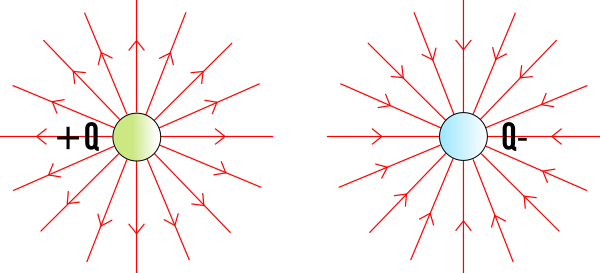
\includegraphics[scale=0.5]{linee-di-campo-elettrico-di-una-carica-puntiforme.png}
\end{center}
\pagebreak
esempio di campo elettrico generato da un dipolo elettrico:
\begin{center}
    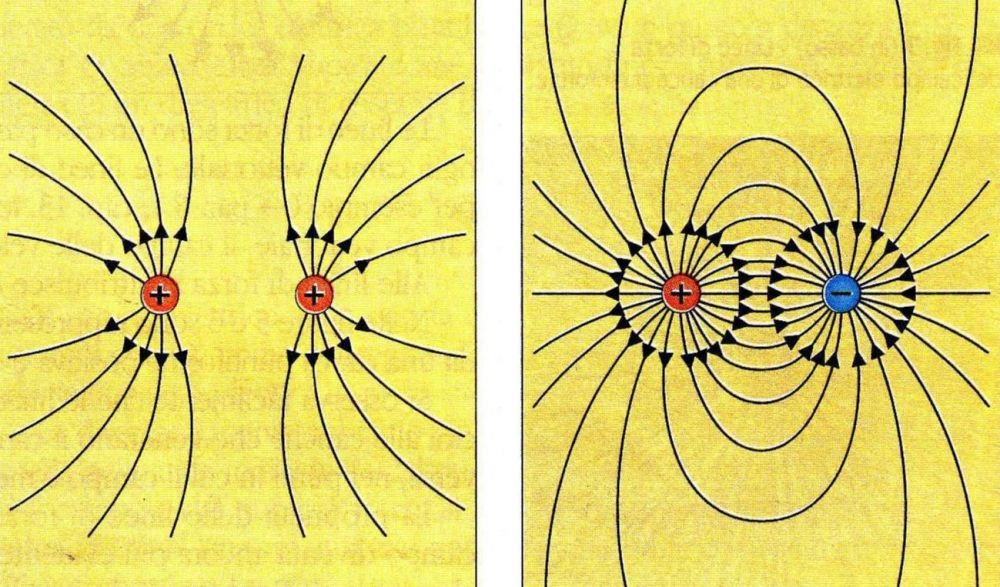
\includegraphics[scale=0.35]{linee_di_forza_di_un_dipolo_elettrico.jpg}
\end{center}


\end{document}


